\documentclass{article}
\usepackage{graphicx} % Required for inserting images
\usepackage{amsmath}
\usepackage{float}
\title{Lesson 2 Homework - Proof Writing}
\author{William Wang}
\date{September 2025}

\begin{document}

\maketitle

\section{}
\subsection{}
We know that the restriction on the domain is just going to be when \(3-x = 0 \implies x \neq 3\). We can solve the range by solving for $y = \frac{2x+1}{3-x}$:
\[3y-xy = 2x+1 \implies x(2+y) = 3y-1 \implies x = \frac{3y-1} {2+y}\]
Hence the range is just \(y \neq -2\). Since the degree of the numerator is equal to the degree of the denominator, we know that there are no slant asymptotes. As \(x \xrightarrow{} 3^-\), we have 
\(\frac{2x+1}{3-x} = +\infty\) and as $x \xrightarrow{} 3^+$, \(\frac{2x+1}{3-x} = -\infty\). Hence there is a vertical asymptote at $x = 3$. Additionally, as \(x \xrightarrow{} \pm \infty\), \(\frac{2x+1}{3-x} =-2\) since the ratio of the leading terms is -2. Hence there is a horizontal asymptote at $y = -2$. 

\[\boxed{\text{Asymptotes are: } y = -2, x = 3}\]
\[\boxed{\text{Domain: All real numbers except } x = 3}\]
\[\boxed{
\text{Range: All real numbers except } y = -2
}\]

\begin{figure}[H]
    \centering
    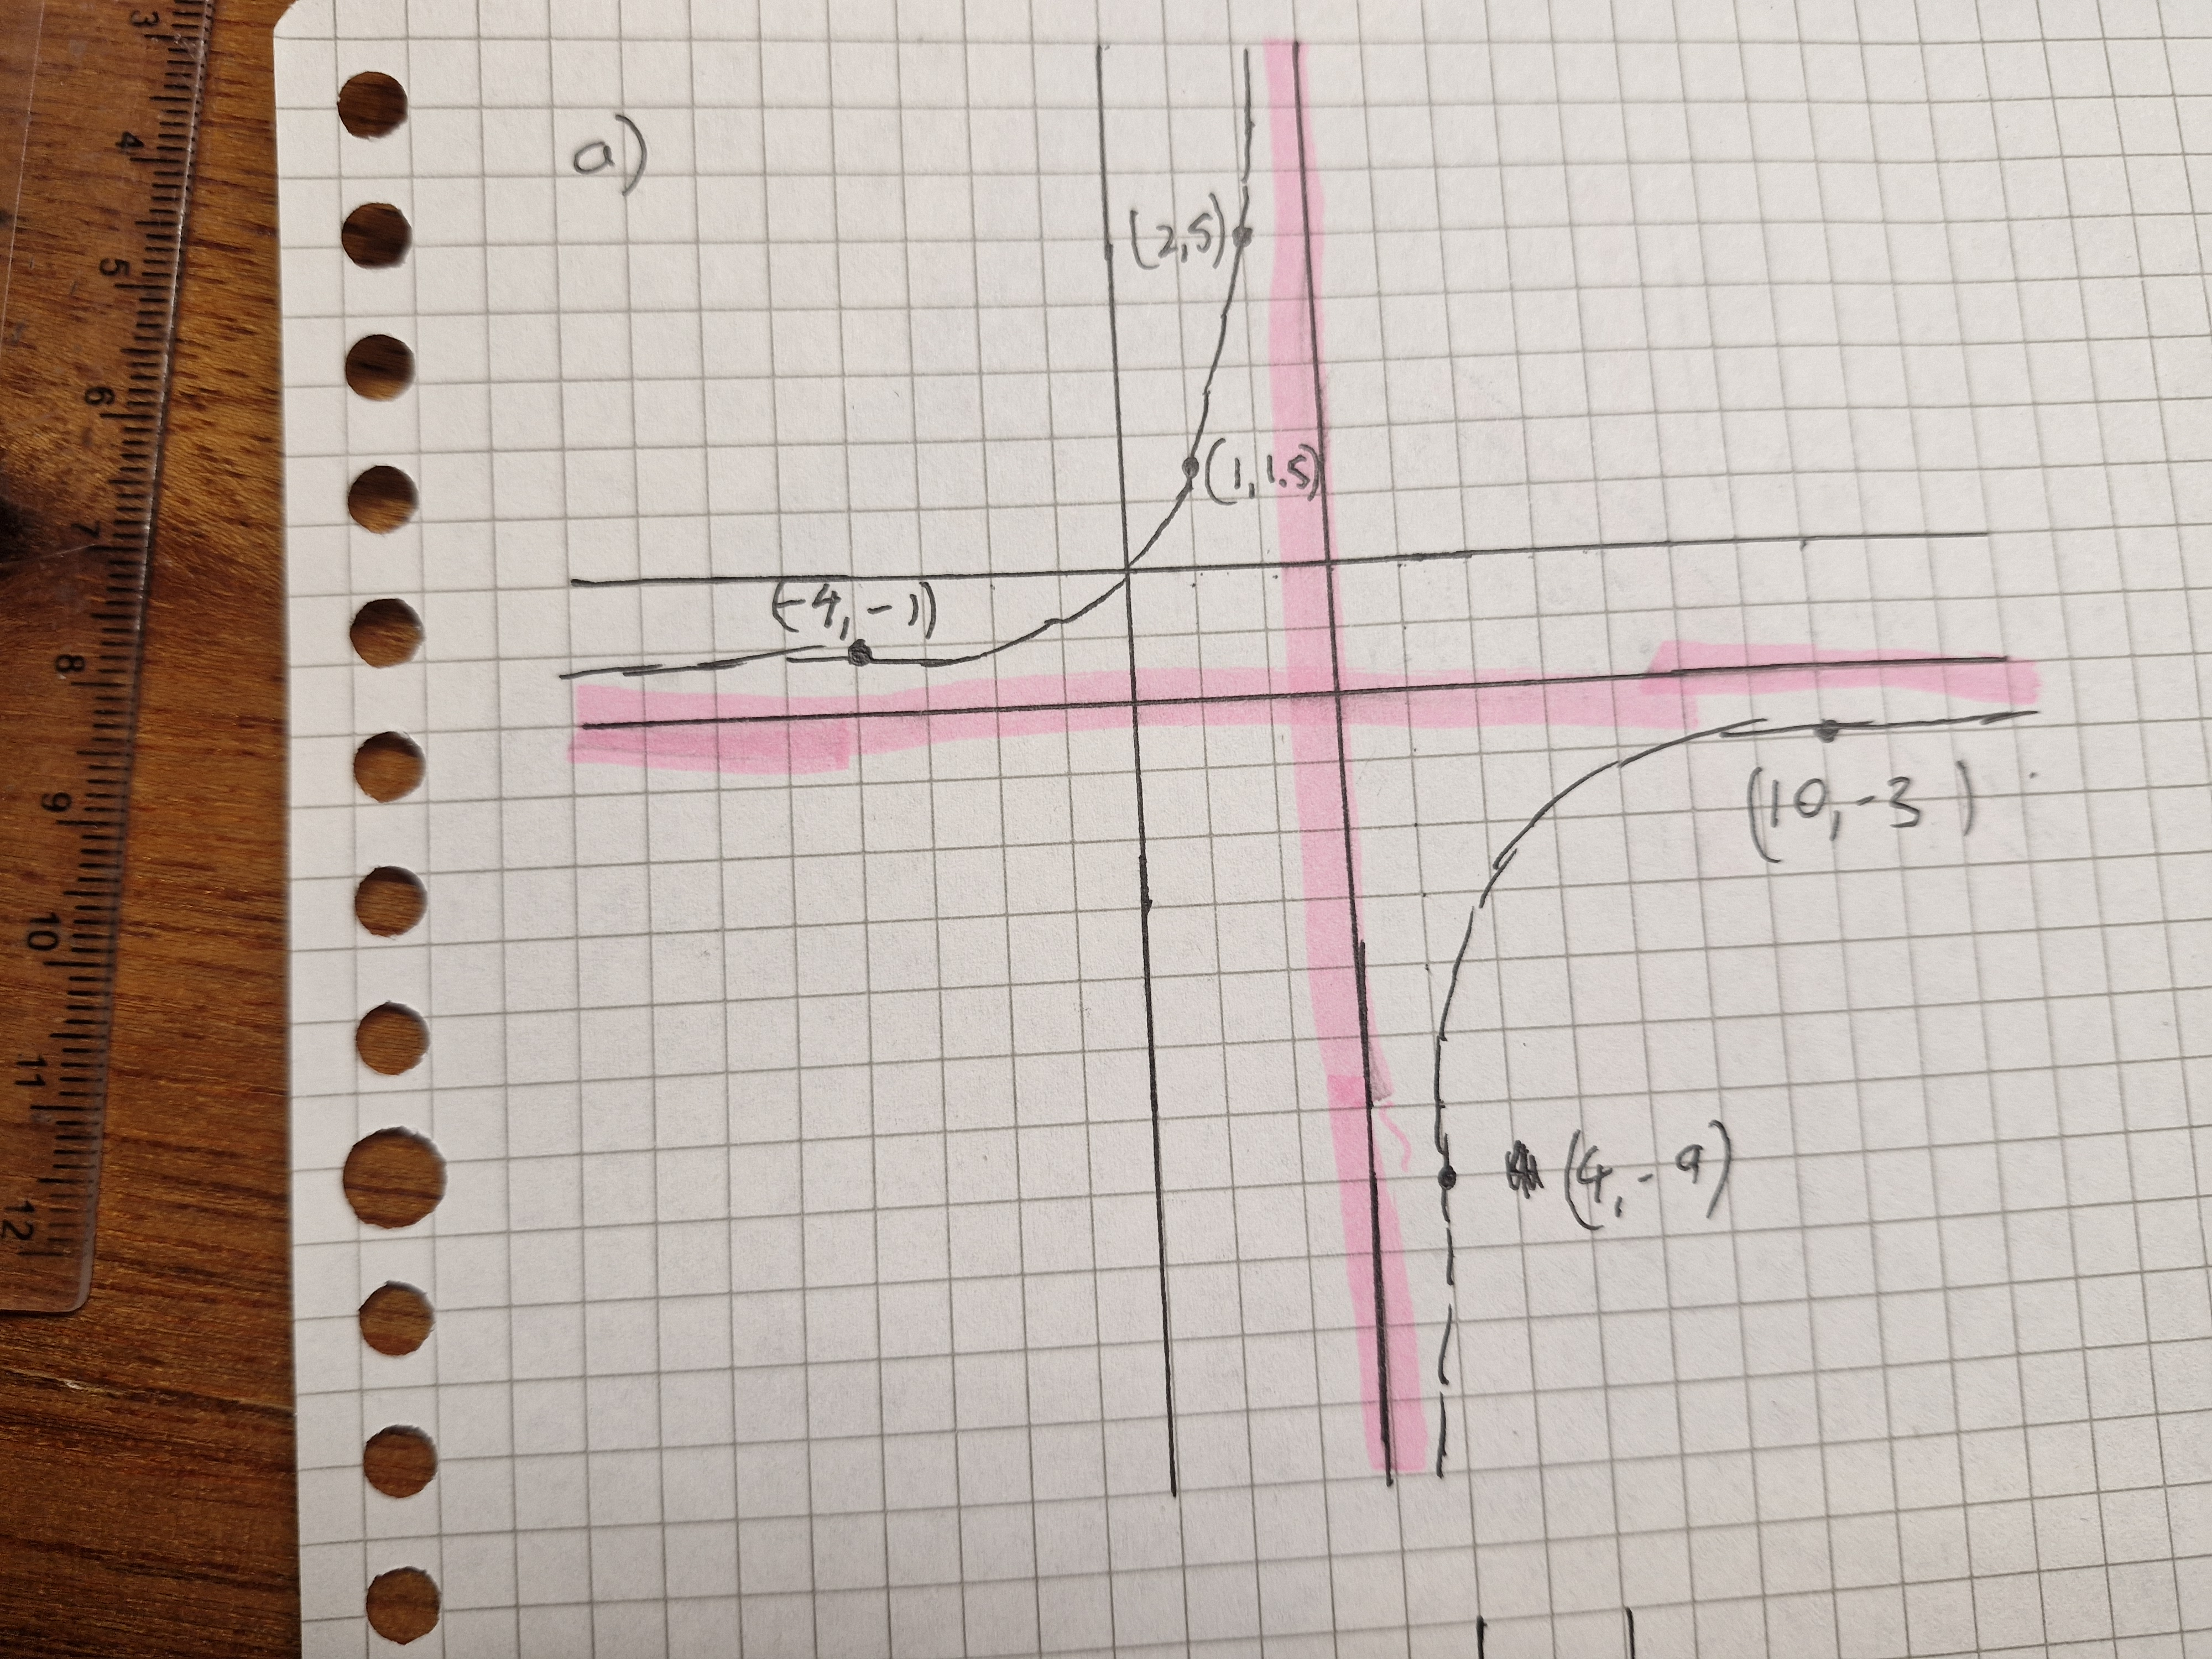
\includegraphics[width=1\linewidth]{1000006499.jpg}
    \caption{Pink lines are the asymptotes (Doesn't actually pass through $(0,0)$)}
\end{figure}

\subsection{}
We know that there is a slant asymptote in this since the degree of the denominator is smaller than the numerator. To find the slant asymptote, we just use long polynomial division to find the remainder and we get that the slant asymptote is \(y = x-2\). We also know the vertical asymptote since we know as \(x \xrightarrow{} 2^+,\frac{x^2-4x+3}{x-2} = +\infty\) and \(x \xrightarrow{} 2^-,\frac{x^2-4x+3}{x-2} = -\infty\). Hence there is a asymptote at $x = 2$. To find the range, we solve for x:
\[\frac{x^2-4x+3}{x-2} = y \implies x^2 - (4+y)x+(3+2y) = 0\]
Since we want the discriminant to be real, we have"
\[y^2+8y+16-12-8y \ge 0 \implies y^2+4 \ge 0\]
We know that $y^2+4 \ge 0$ is always true by the trivial inequality. Hence the range is all real values.
\[\boxed{\text{Asymptotes are: } y = x-2, x = 2}\]
\[\boxed{\text{Domain: All real numbers except } x = 2}\]
\[\boxed{
\text{Range: All real numbers}}\]

\begin{figure}[H]
    \centering
    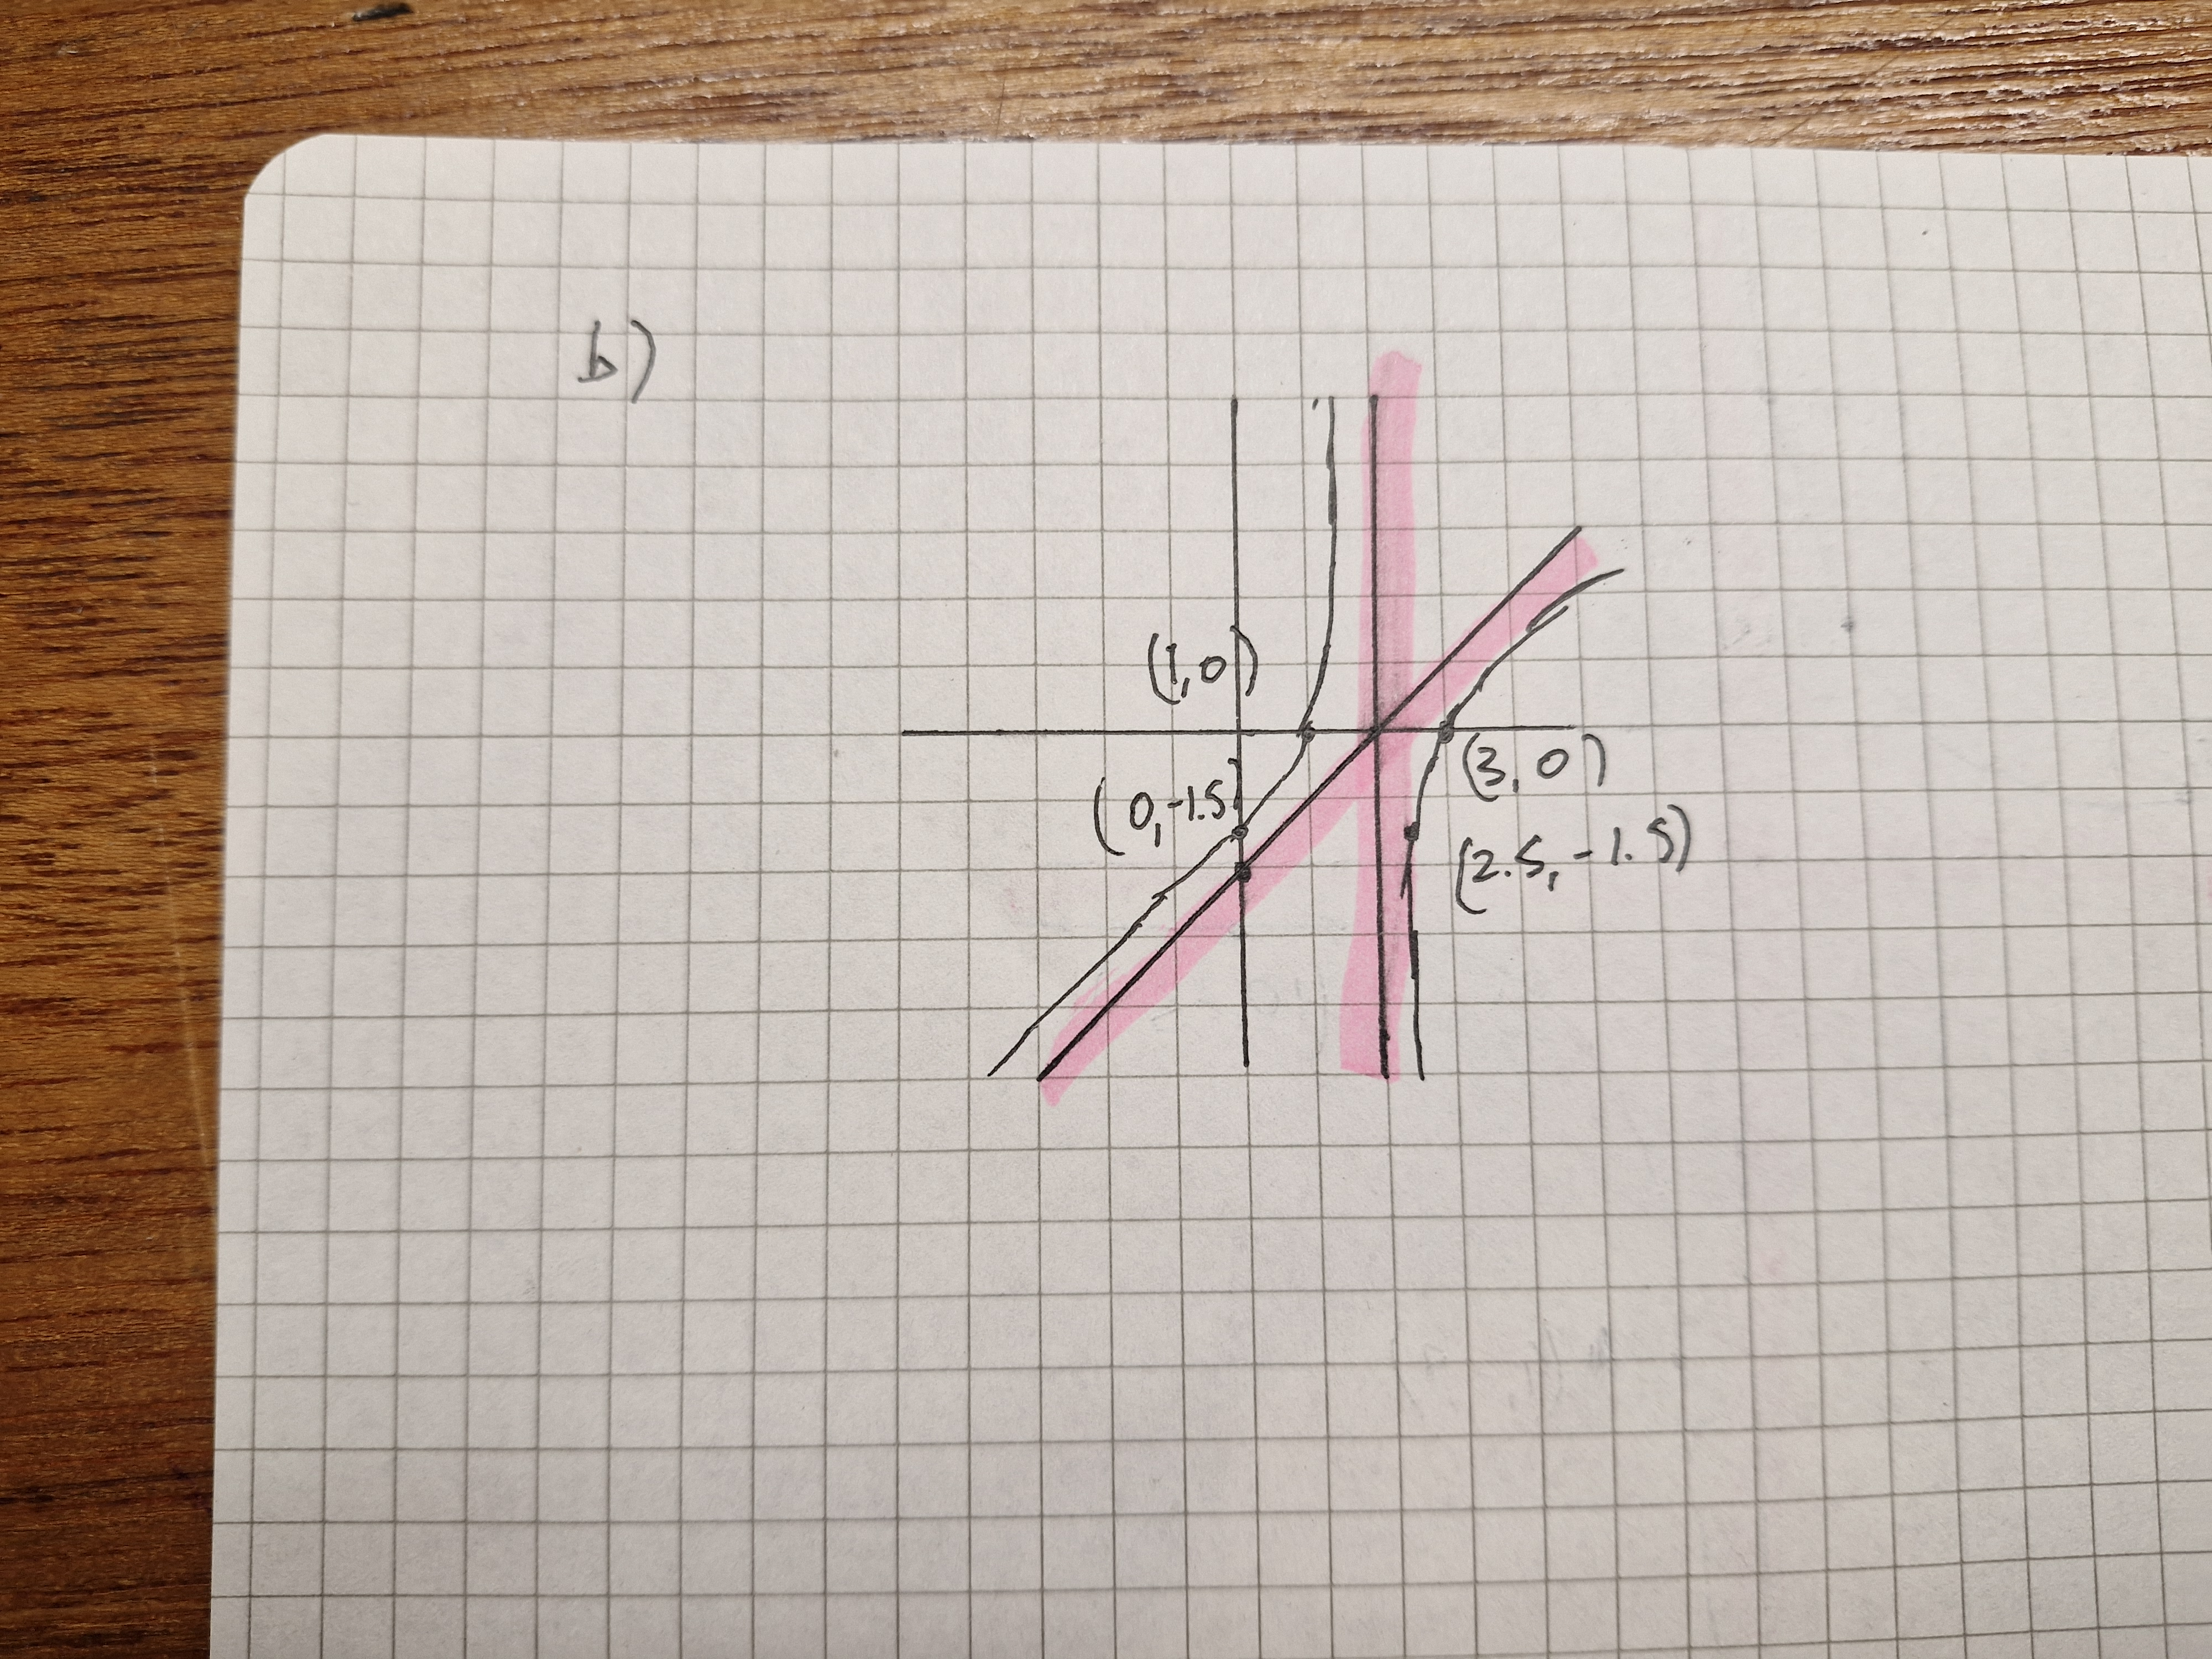
\includegraphics[width=1\linewidth]{1000006500.jpg}
    \caption{Pink lines are the asymptotes}
\end{figure}
\section{}
Since we have 
\[y = \frac{a_n x^n + a_{n-1} x^{n-1} ... a_0}{b_n x^n + b_{n-1} x^{n-1}...b_0}\]
We can divide the top and the bottom by $x^n$, then we have
\[
f(x) = \frac{a_n + \frac{a_{n-1}}{x} + \cdots + \frac{a_0}{x^n}}
             {b_n + \frac{b_{n-1}}{x} + \cdots + \frac{b_0}{x^n}}.
\]
Since asymptotes deal with values where the $x$ values are closer to closer to infinity, we know that as $x \xrightarrow{} \infty$ each of the fraction terms in the denominator and numerator approach 0. Additionally when $x \xrightarrow{} -\infty $, each of the fractional terms in the numerator and the denominator also approach 0 from the negative direction. Hence, we know that the horizontal asymptote is
\[y = \frac{a_n}{b_n}\]

\section{}
We can find the range of $f(x)$ by solving for $x$. 
\[\frac{x^2-2x+3}{x^2+2x-3 }= y \implies = yx^2+2xy-3y = x^2-2x+3\]
\[\implies (y-1)x^2 + (2y+2)x - (3+3y) = 0\]
Since y has to be real, we can use the discriminant:
\[(2y+2)^2 + 4(3+3y)(y-1) \ge 0 \implies 4y^2+8y+4 + 4(3y^2-3) \ge 0\]
\[\implies 16y^2+8y-8 \ge 0 \implies 2y^2+1y-1 \ge 0  \]
Then we know that the
\[\text{Range} \in (-\infty, -1], [1/2, \infty) \]
\begin{figure}[H]
    \centering
    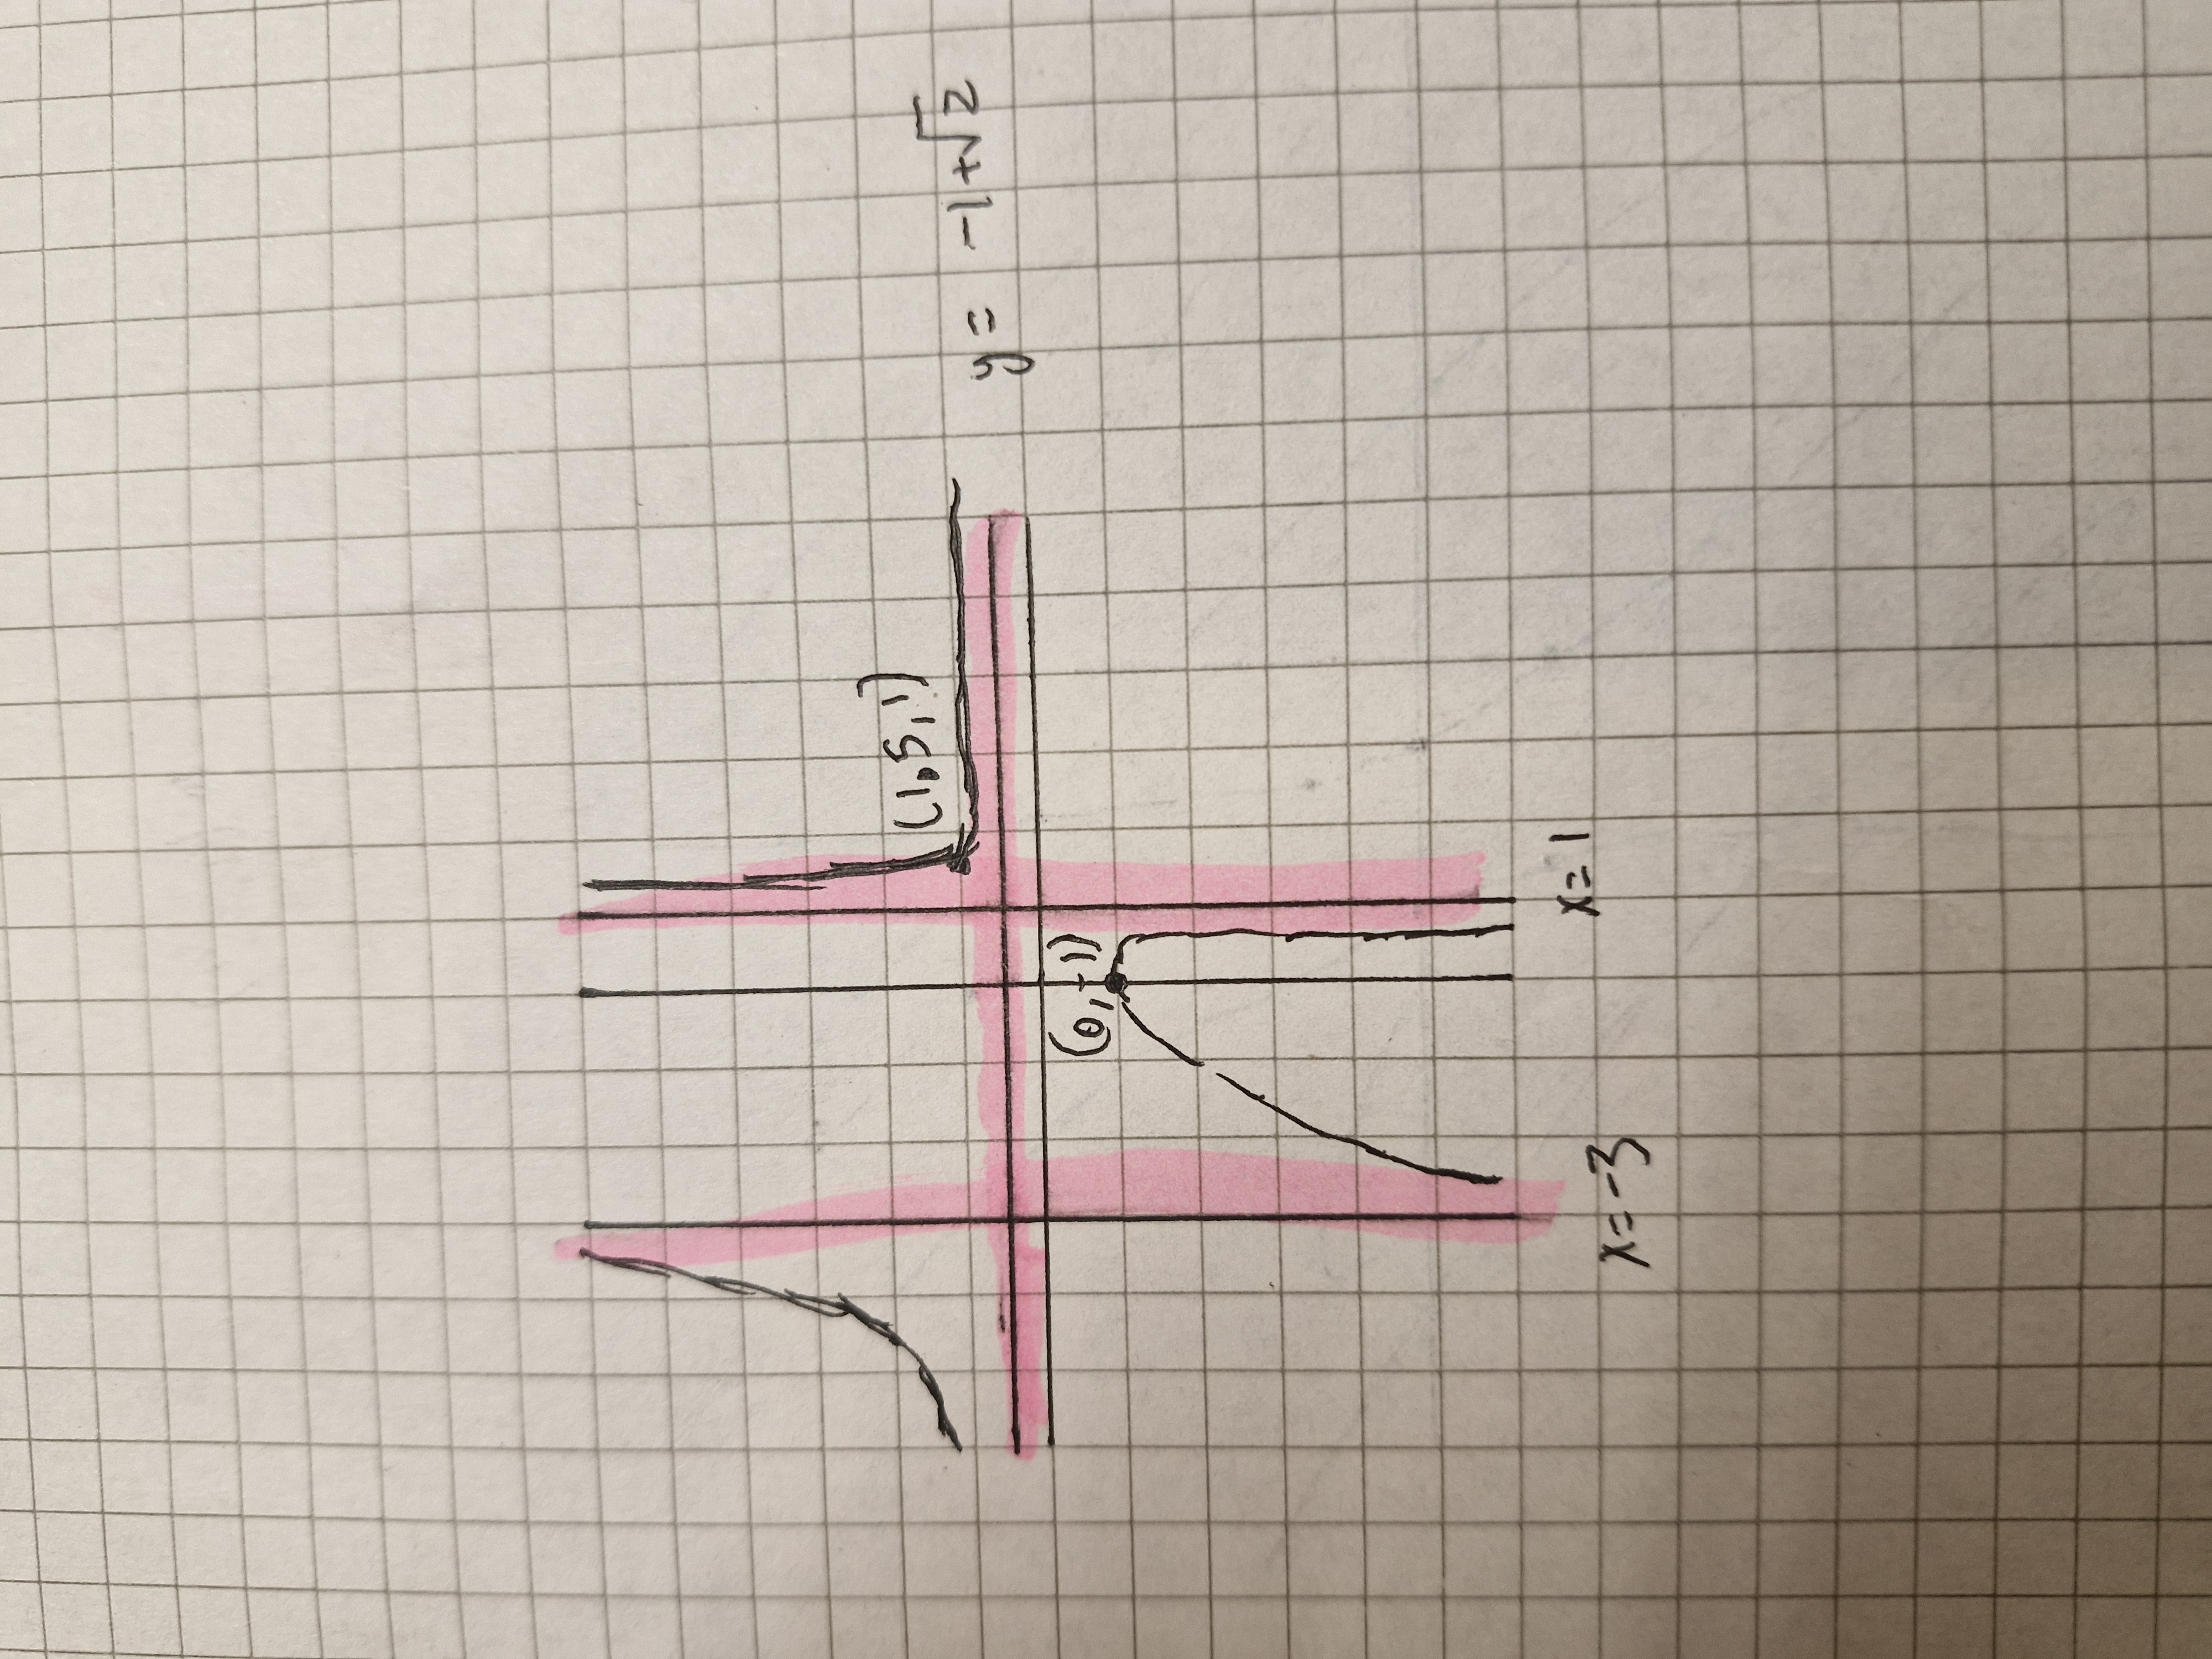
\includegraphics[width=1\linewidth]{1000006501.jpg}
    \caption{Pink lines are asymptotes}
\end{figure}


\end{document}
